\section{Template Extraction}
Before template images can be extracted for cross-correlation, they must first be
identified in the source spectrograms.
If matching results are to be consistent, spectrograms must undergo
noise reduction and segmentation.
This section details the mechanisms developed for preprocessing spectrogram
images and filtering segments so that only the relevant templates are included for
extraction.

Each spectrogram is processed in sequence using functionality provided by the
OpenCV \parencite{opencv_library} library, and immediately stored on disk.
Parallelisation is possible here, but the computational cost of this stage is
not large enough to have justified sparing development time on this aspect.

\section{Spectrogram Preprocessing}\label{sec:preproc}

Before any features may be extracted, their boundaries must be found.
This is a non-trivial problem due to undesireable noise and recording artefacts
present in each spectrogram.
The problem is considerably worsened by the inconsistency of these from sample
to sample.

The figure below shows an example of a noisy spectrogram.
Notice how the background noise makes it difficult to find the exact boundary of
some of the vocalisations.

show sgram with noise

Even with the quality prefiltering done when downloading recordings from
Xeno-canto, such noise levels remain common.

Because a high number of samples is required for our approach, we developed an
automatic noise reduction stage.
Standard computer vision techinques for noise reduction were used, as well as
techniques for discrete object identification.
A filter is first applied to the spectrogram, which reduces the noise in the
image by smoothing just enough until granular noise is reduced sufficiently (figure x).
The image is then thresholded using an adaptive thresholding algorithm (figure x).
We used adaptive thresholding due to the pixel intensity inconsistencies
throughout some of the spectrogram images.
Further noise reduction is then performed using erosion and dilation which
removes small segments and joins pixel groups which are in close proximity to
each other (figure x).

--\\

global parameters for sweeping noise reductions are suboptimal, what may work
for one recording might not work for another.

yet this is what we do, works ok, specific values were found through trial and
error.

objective is to process spectrograms to find contiguous blobs with similar
scope, that is, either phrases or individual vocalizations.

Some noise reduction steps are semi-automatic, such as adaptive thresholding.

a better approach would be to operate on a per-spectrogram basis, to find the
optimal parameters for each.

This is a non trivial problem.

conceptually the noise reduction algorithm would perform some parameter search
with a heuristic based on the dimensions and quantity of contiguous blobs, with
the aim of reducing the number of small blobs which may resemble noise or disjoint
parts of a single vocalization or segment.

The target scope should be specifiable, so that either individual vocalizations
or complete segments or songs could be extracted.

In some cases it might not be possible to achieve total correct segmentation.

Since different birds have different lengths for specific sounds or parts of song,
the spectral dimensions can not be generalized.
This means that each species will have different aims for quantity and dimensionality,
which must be constructed either by manual input or some feedback mechanism.

a feedback system can then be used to determine which type of segmentation works
best by filtering to various sizes and measuring the accuracy obtained after
classification.


\subsection{Basic Selection and Extraction}\label{sec:template_select}
Given optimal results the segments represent parts of song at the desired
granularity.
This is often not the case however.
Noise may persist after preprocessing, and new deformations may appear, such as
incorrectly joined or incomplete segments.

Some effort is taken to reduce the number of undesireable templates after
preprocessing.
In addition to noise, undesireable templates include extremely specific or
extremely generalised templates.

For example, if a sound is featured in a single instance of bird song, but not
in any other recording of songs of that species, then it is an extreme outlier,
which may occur due to a bird's individual expression or originate from external
sources.
It is non trivial to detect outliers during feature extraction, but because
random forests are generally insensitive to this type of error, we do not
account for these at this stage.

Generalised, or weak templates are easier to detect.
Such templates will have a very faint structure (low contrast), or a complete
lack of structure.
These may be analysed directly and ignored, as they are likely to correlate,
although very weakly, to the majority of spectrograms irrespective of the
species.

Although these rejections bring a theoretical boost to classifier accuracy and
performance, they mainly benefit performance by reducing the number of
cross-correlations computed.

\begin{figure}[h]
  \centering
  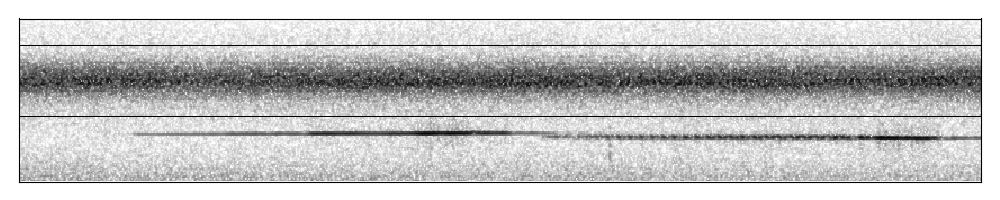
\includegraphics[width=1\textwidth]{large_template}
  \caption{Spectrogram featuring rejected extremely large noise segment}
  \label{fig:bad_select}
\end{figure}

\begin{figure}[h]
  \centering
  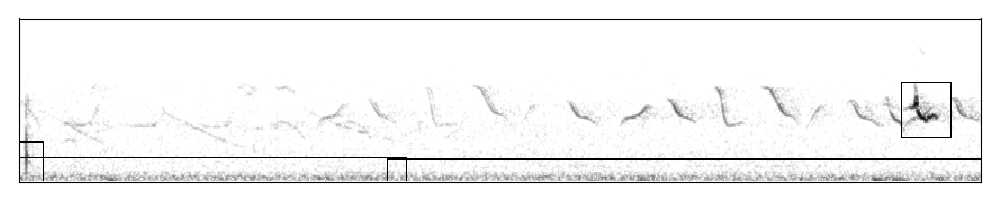
\includegraphics[width=1\textwidth]{bad_select}
  \caption{Spectrogram featuring erronously rejected weak templates}
  \label{fig:bad_select}
  %used XC36327
\end{figure}

\subsubsection{Selection mechanism}
Complete elimination of all undesireable features is impossible without also
removing desireable features.
A balance must therefore be struck, in both preprocessing and selection stages.
Performing selection manually is infeasable given the quantity
of pixel segments.
Selection is therefore done automatically by considering the dimensionality and
pixel values of each template.
Results are shown in Figure~\ref{fig:template_select_effects}\\

Templates with the following properties are automatically rejected:
\begin{itemize}[noitemsep]
  \item \textbf{Area smaller than 50 pixels:} Templates with small dimensions
    are too small to be of any significance and are most likely noise or
    artefacts from preprocessing;

  \item \textbf{Area larger than 10000 pixels:} Templates with extremely large
    dimensions are most likely artefacts from preprocessing, high intensity
    noise or continuous external noises.
    It is possible for sections of song to be merged together into a single
    pixel region due to preprocessing errors.

  \item \textbf{Maximum template intensity lower than average intensity of the
    spectrogram:}
    Low maximum intensity is an indicator background or baseline noise.
    This filter eliminates some of these templates, however not very well.
    Local variance may be a better property to test for, but this has not been
    explored.
\end{itemize}

\begin{figure}[!htb]
  \centering
  \begin{subfigure}[b]{1.0\textwidth}
    \centering
    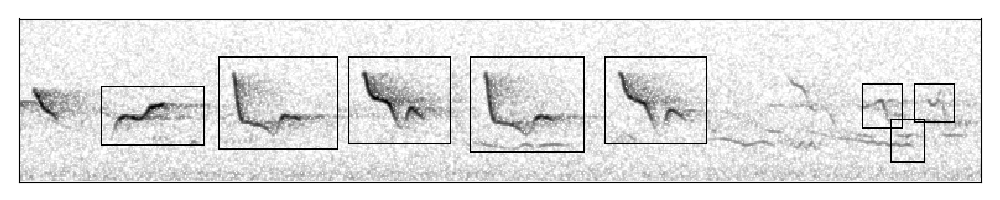
\includegraphics[width=1\textwidth]{accept}
    \caption{}
  \end{subfigure}
  \begin{subfigure}[b]{1.0\textwidth}
    \centering
    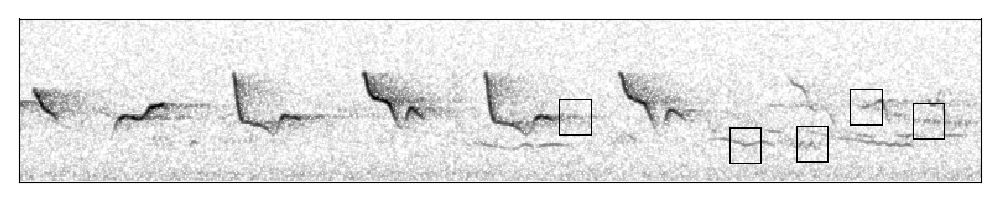
\includegraphics[width=1\textwidth]{reject}
    \caption{}
  \end{subfigure}
  \caption{A noisy spectrgoram showing accepted (a) and rejected (b) templates}
  \label{fig:template_select_effects}
\end{figure}

\subsubsection{Extraction mechanism}\label{sec:extract}

A bounding box is computed for the contours of each segment, which is then used
to extract a template from the original spectrogram image.
Once selection is performed for a particular pixel region, it's bounding box is
expanded by 10 pixels in each direction, and that region is extracted from the
original, unprocessed spectrogram.
This forms a single template.
The template is then blurred using a Gaussian filter with a sigma of 1.5.

Blurring the template allows us to reduce its size, which brings performance
boosts to template matching.
Blurring the template also improves it's generality, which makes matches more
likely.
Care is taken to ensure that templates do not become overly generic, resulting
in ambiguity.
The same operation is made to the spectrograms subject to cross-correlation
mapping for consistency.

\subsection{Advanced Template Elimination}
It is desireable to reduce the template count further.
This can be made possible by recognizing correlations between candidate templates.
This subsection outlines some speculative methods for
selecting better templates.

\subsubsection{Spatial inclusion}
Imperfections in the preprocessing mechanism leads to errorneous pixel segments.
Incorrect gaps, joins and other inconsistencies in structure persist or
materialise.
If ignored, these are extracted along with valid templates.
If infrequent, the additional templates will factor less as an accuracy penalty,
and more as a performance issue.

In many of these cases, one template's bounding box intersects or is contained
entirely within another template's bounding box as shown in
Figure~\ref{fig:segment_intersect_a}.
These errors can be corrected by taking the bounding box of their unions.
In contrast, Figure~\ref{fig:segment_intersec_b} shows that this does not always
work, and result in large, incorrect groupings.

\begin{figure}[!htb]
  \centering
  \begin{subfigure}[h]{0.5\textwidth}
    \centering
    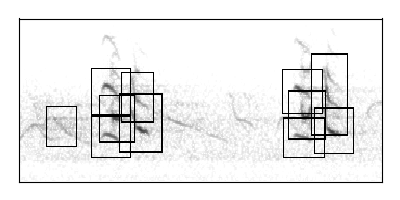
\includegraphics[width=1.0\textwidth]{spatial_fix}
    \caption{}\label{fig:segment_intersect_a}
  \end{subfigure}%
  \begin{subfigure}[h]{0.5\textwidth}
    \centering
    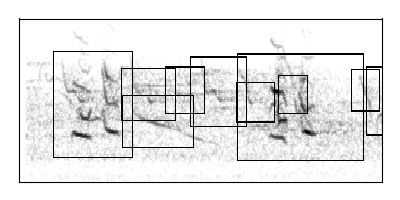
\includegraphics[width=1.0\textwidth]{spatial_unfix}
    \caption{}
    \caption{}\label{fig:segment_intersect_b}
  \end{subfigure}
  \caption{Example of errorneous segmentations correctable (a) and incorrectable (b)
  by merging their bounding boxes}
  \label{fig:segment_intersect}
\end{figure}

\subsubsection{inter-template correlation}
As expected, templates will have some level of inter-correlation.
This leads to a database of many hundreds or thousands of very similar templates.
Merging these in some form has been considered but not approached.
This would benefit performance dramatically, but it is most likely to cause
a noticeable dip in accuracy.
For this to succeed, the result of the merge must represent all related templates
equally, and it is clear that this would not be as accurate as individual
templates.

It can also be argued that templates with little to know intercorrelation may be
independent anomalies, such as noise or external signals irrelevant to the
subject species.

\subsubsection{Species-specific template statistics}
It may be possible to use information regarding average dimensionality and mean
frequency information to determine the relevance likelyhood of a particular template.
Such metrics require an existing set of validated templates, which may be gathered
by filtering a non discriminated set of templates by their measures importances.

Figure~\ref{fig:bandlimit} shows how the birdx song doesn't use vocalisations
under 123 Hz.

\begin{figure}[!htb]
  \centering
  \caption{Example of a bird song with a principal frequency range}
  \label{fig:bandlimit}
\end{figure}
